\subsection{Quelques leçons des expériences de Stanley Milgram}

	\paragraph{Le protocole expérimental et ses résultats}

	Des personnes sont convoquées à Yale et constituent des binômes élève-professeur.
	Le sujet “professeur” doit infliger à un sujet des décharges électriques avec une tension croissante jusqu'à 450 V lorsque l'élève (complice) répond mal aux questions posées.
	Le sujet a été mené avec 536 sujets (professeurs).
	Initialement, 65\% des sujets la poursuivent jusqu'au bout.
	Le résultat est le même avec des binômes masculins et féminins.

	\paragraph{Les facteurs influençant l'administration de la punition}

	Milgram a mené 16 variantes.
	Dans l'une d'entre elle, où Yale est remplacé par des bureaux privés et l'étude semble commandité par une entreprise sérieuse, mais sans la caution de la science et de Yale, il y a encore 47,5\% des sujets qui vont jusqu'au bout.
	Dans une autre le professeur peut voir la victime et le taux d'individus allant jusqu'au bout est alors de 40\%.
	Dans une autre encore, la victime doit avoir la main sur une plaque pour être électrocutée et l'on demande au “professeur” de lui remettre la main sur la plaque, établissant ainsi un contact physique.
	Le taux est alors de 30\%.

	\paragraph{La question de la responsabilité}

	Lorsqu'on demande au sujet d'indiquer comment se fait selon eux la répartition de la responsabilité, voici ce qu'ils répondent :

	\vspace{0.3cm}
	\begin{tabular}{|r|rrr|}
	\hline
	Responsabilité & Expérimentateur & Moi & Élève \\
	\hline
	Sujets rebelles & 39\% & 48\% & 13\% \\
	\hline
	Sujets obéissants & 38\% & 36\% & 26\% \\
	\hline
	\end{tabular}
	\vspace{0.3cm}

	Lorsque la tâche d'abaisser la manette est déléguée à un autre, le taux d'individus qui vont jusqu'au bout est de 92,5\%.
	Lorsque la responsabilité est diluée il y a donc plus de personnes qui vont jusqu'au bout.

	Si l'expérimentateur quitte la pièce et communique par téléphone, la part de ceux qui vont jusqu'au bout tombe à 20,5\%. Ce qui se passe est que les sujets mentent et prétendent infliger de fortes décharges alors qu'ils se limitent en fait aux premiers leviers.

	Cela rejoint les thèses de Hannah Harendt élaborées à l'issue du procès Eichmann.
	Elle y affirme que Eichmann est plus un fonctionnaire zelé qu'un réel sadique raciste.
	Harendt forge alors l'expression de “banalité du mal”.

	\paragraph{La question de la résistance à l'autorité : le point de vue de Serge Moscovici}

	L'explication avancée par Serge Moscovici est que la donnée fondamentale qui amène à une soumission est l'isolement.
	En effet, dans une variante où un second professeur complice commence à refuser d'infliger les décharges, le sujet va tendre fortement à stopper lui-même.

	Une autre expérience de Milgram (15\up{e}) met en jeu deux expérimentateurs, l'un décide à partir de 150 V et des premiers signes de souffrances qu'il ne souhaite pas poursuivre cette expérience.
	L'autre souhaite poursuivre et reste sur place, mais une faille est découverte dans le processus de légitimation.
	La soumission chute alors brutalement : sur un petit échantillon, aucun ne va jusqu'au bout.

	Certains sujets s'enquièrent alors de la hiérarchie entre les scientifiques.

	\paragraph{Résumé.}
	Milgram : la capacité d'obéissance à l'autorité varie d'abord en fonction des circonstances : les actes sont moins la conséquence d'un trait de caractère permanent des individus que le résultat de l'interaction entre un individu et un dispositif de soumission.

	Harendt : la soumission dépend du degré de déresponsabilisation obtenue chez le sujet.
	En rejetant la responsabilité sur l'autorité et / ou la victime, l'individu peut finalement participer à un crime en tant que « simple rouage ».
	
	Moscovici : la résistance à la soumission se renforce grâce au soutien que l’individu peut trouver chez d’autres personnes, ou grâce aux failles qu’il peut découvrir dans le processus du légitimation de l’autorité.

\subsection{Le contrôle des prisonniers}

	Le gardien cherche à rendre les prisonniers aussi dociles que possible.

	\paragraph{Les prisonniers américains en Corée : Robert Cialdini.}

	Dans son ouvrage \textit{Influence}, Robert Cialdini, prend l'exemple de la guerre de Corée (1950-1953).
	Les chinois (du côté Nord-coréen) évitaient la douleur et mettaient en place des procédés de manipulation psychologique assez avancés.
	Grâce à ses techniques, les prisonniers se dénonçaient entre eux.
	Les plans d'évasions étaient ainsi très souvent déjoués et les fugitifs très facilement retrouvés.

	On commençait par exemple par demander à un soldat de faire une déclaration très légèrement anti-américaine, ou légèrement pro-communiste.
	La collaboration des prisonniers allait alors croissante : on leur demander d'indiquer ce qui n'allait pas aux États-Unis, d'en discuter...
	On leur faisait alors écrire, en allant dans un sens pro-communiste.
	Les prisonniers devaient ensuite assumer la responsabilité de ces actes, s'y enchaînant ainsi malgré eux.

	Une expérience a été menée pour voir si les soldats avaient vraiment pu être tournés en faveur du communisme.
	On a demandé à un échantillon de personnes de lire un texte en faveur de Fidel Castro écrit par un soldat américain.
	Dans le premier cas on leur disait que l'auteur avait écrit librement le texte, et dans l'autre qu'il y avait été “instamment prié”.
	Même dans le second cas il s'est alors avéré que le lecteur pensait que l'auteur pensait en partie ce qu'il écrivait.

	Les chinois organisaient également des concours de texte politique, avec des prix modestes mais sous forme de marchandises non inintéressantes.
	Les prisonniers pouvaient alors gagner en défendant la position de leur pays, mais avec quelques concessions.
	Pour gagner, les prisonniers ont commencé d'eux-mêmes à gauchir leurs textes.

	\paragraph{Le Panoptique : Michel Foucault (\textit{Surveiller et punir})}

	Le panoptique est un type d'architecture carcérale inventée par le britannique Jeremy Bentham.
	Le bâtiment est constitué d'un grand bâtiment en anneau, avec un large espace central et de nombreuses cellules dans la paroi.
	Chaque ouverte est ouverte des deux côtés : sur l'intérieur, et sur l'extérieur de l'anneau, ce qui permet à la lumière de traverser la structure.
	Au centre de l'anneau se trouve une petite tour qui permet de surveiller l'ensemble des prisonniers.
	
	\begin{figure}[htp]
	\centering
	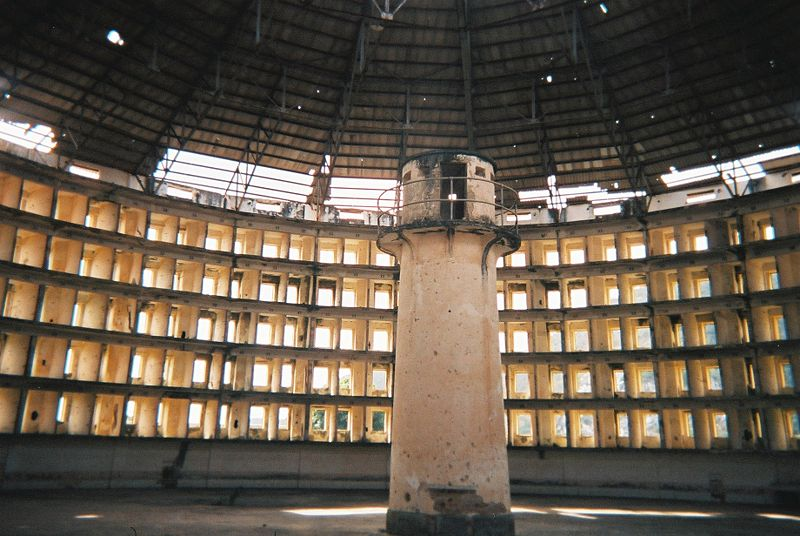
\includegraphics[scale=0.5]{panoptique.jpg}
	\caption{L'intérieur de la prison Presidio Modelo, à Cuba, construite sur le modèle du panoptique}
	\end{figure}

	Le prisonnier ne sait alors pas quand il est observé.
	Il n'y a pas d'angle mort, personne ne peut se cacher.
	Ainsi le surveillant abandonne une partie du travail aux surveillés.
	On limite donc le nombre de surveillant nécessaires et on rend les prisonniers plus dociles.

	Si Foucault s'y intéresse c'est parce que, selon lui, cette structure possède une capacité d'oppression qui va bien au-delà du monde carcéral.
	Pour lui le Panoptique est emblématique d'une tendance moderne : remplacer la contrainte violente des dispositifs de contrôle à distance, en passant à travers la généralisation des dispositifs de surveillance.

	Extensions possibles de la thèse de Foucault :
	\begin{itemize}
		\item Les open-spaces. Aujourd'hui beaucoup de cadres et employés sont placés sur des plate-formes open-spaces. Les bureaux séparés ne sont plus que pour les plus haut gradés.
			Les salariés exercent alors une surveillance des uns les sur autres.
		\item Le bracelet électronique. Depuis 1997 un magistrat peut demander un placement d'un bracelet et, depuis la loi Dati, ce dispositif est étendu à des individus ayant purgé leur peine mais considérés comme dangereux.
			Les motivations financières n'y sont sans doute pas étrangères et cela offre des avantages pour le prisonnier.
			Il dématérialise encore plus la contrainte pesant sur le condamné et semble transformer le prisonnier en “surveillé”.
		\item Les caméras de surveillance.
	\end{itemize}
